\subsubsection{ΠΕΡΙΠΤΩΣΗ ΧΡΗΣΗΣ 2: Καταγραφή τιμής ενός προϊόντος από εθελοντή}
\subsubsubsection{Χρήστες (ρόλοι) που εμπλέκονται}
Ο μόνος που εμπλέκεται σε αυτήν την περίπτωση χρήσης είναι ο εθελοντής που επιθυμεί να πραγματοποιήσει την καταγραφή της πλέον πρόσφατης τιμής ενός προϊόντος κάποιου πρατηρίου υγρών καυσίμων.
\subsubsubsection{Προϋποθέσεις εκτέλεσης}
Για την επιτυχή εκτέλεση του παραπάνω σεναρίου χρήσης, θα πρέπει να ικανοποιούνται οι παρακάτω προϋποθέσεις:
\begin{enumerate}
	\item Σύνδεση στο διαδίκτυο
	\item Η βάση δεδομένων του backend είναι online
	\item Η διαδικτυακή διεπαφή λειτουργεί
	\item Ο χρήστης πρέπει να είναι συνδεδεμένος στο λογαριασμό του
	\item Το κατάστημα το οποίο διαθέτει το προϊόν να βρίσκεται στη βάση
	\item O τύπος του προϊόντος να είναι διαθέσιμος
\end{enumerate}
\subsubsubsection{Περιβάλλον εκτέλεσης}
Το περιβάλλον στο οποίο εκτελείται η περίπτωση χρήσης είναι η διαδικτυακή διεπαφή χρήστη, είτε από κάποιο φυλλομετρητή, είτε από κάποιο smartphone.
\subsubsubsection{Δεδομένα εισόδου}
Σαν δεδομένα εισόδου θεωρούνται τα στοιχεία που δίνει ο εθελοντής-χρήστης προκειμένου να πραγματοποιηθεί το login, καθώς και τα στοιχεία που απαιτούνται για την εν λόγω καταχώρηση. \\
Οι συνθήκες εγκυρότητας για τα παραπάνω είναι η ταυτοποίηση του χρήστη και η ύπαρξη του συγκεκριμένου πρατηρίου υγρών καυσίμων (μέσω της βάσης δεδομένων). Επίσης, η συσκευή που χρησιμοποιεί ο χρήστης να είναι συμβατή με την κωδικοποίηση κειμένου του συστήματος (\texttt{utf8}).\\
Ως δεδομένο εξόδου θεωρείται η ενημέρωση της βάσης δεδομένων για την τιμή του προϊόντος που καταχώρησε ο χρήστης. \\
Οι συνθήκες εγκυρότητας για το παραπάνω είναι ο χρήστης να συμπλήρωσει όλα τα απαραίτητα πεδία για την επιθυμητή καταχώρηση καθώς και η ύπαρξη του προϊόντος στη βάση δεδομένων.
\subsubsubsection{Παράμετροι}
Καταγραφή παραμέτρων και συνθηκών εγκυρότητας αυτών
\subsubsubsection{Αλληλουχία ενεργειών - επιθυμητή συμπεριφορά}
Τα βήματα για την πραγματοποίηση της καταχώρησης είναι τα εξής:
\begin{enumerate}
	\item Είσοδος στην ιστοσελίδα
	\item Επιλογή του sign in
	\item Εισαγωγή στοιχείων για την πραγματοποίηση του login
	\item Εμφάνιση homepage, η οποία θα περιέχει το χάρτη
	\item Επιλογή πρατηρίου από τον χάρτη
	\item Επιλογή κουμπιού καταχώρησης τιμής στο pop-up που εμφανίζεται από την επιλογή του πρατηρίου
	\item Συμπλήρωση απαραίτητων πεδίων για την καταχώρηση της τιμής
\end{enumerate}
Το αντίστοιχο διάγραμμα είναι το \ref{fig:User_Login}

\subsubsubsection{Δεδομένα εξόδου}
Εξετάζεται η περίπτωση προσθήκης προϊόντος στο διάγραμμα \ref{fig:User_Add_Product}.

% \subsubsubsection{Παρατηρήσεις}
% Ο,τι δεν εντάσσεται στα προηγούμενα, εφόσον υπάρχει



\begin{figure}[H]
    \centering
    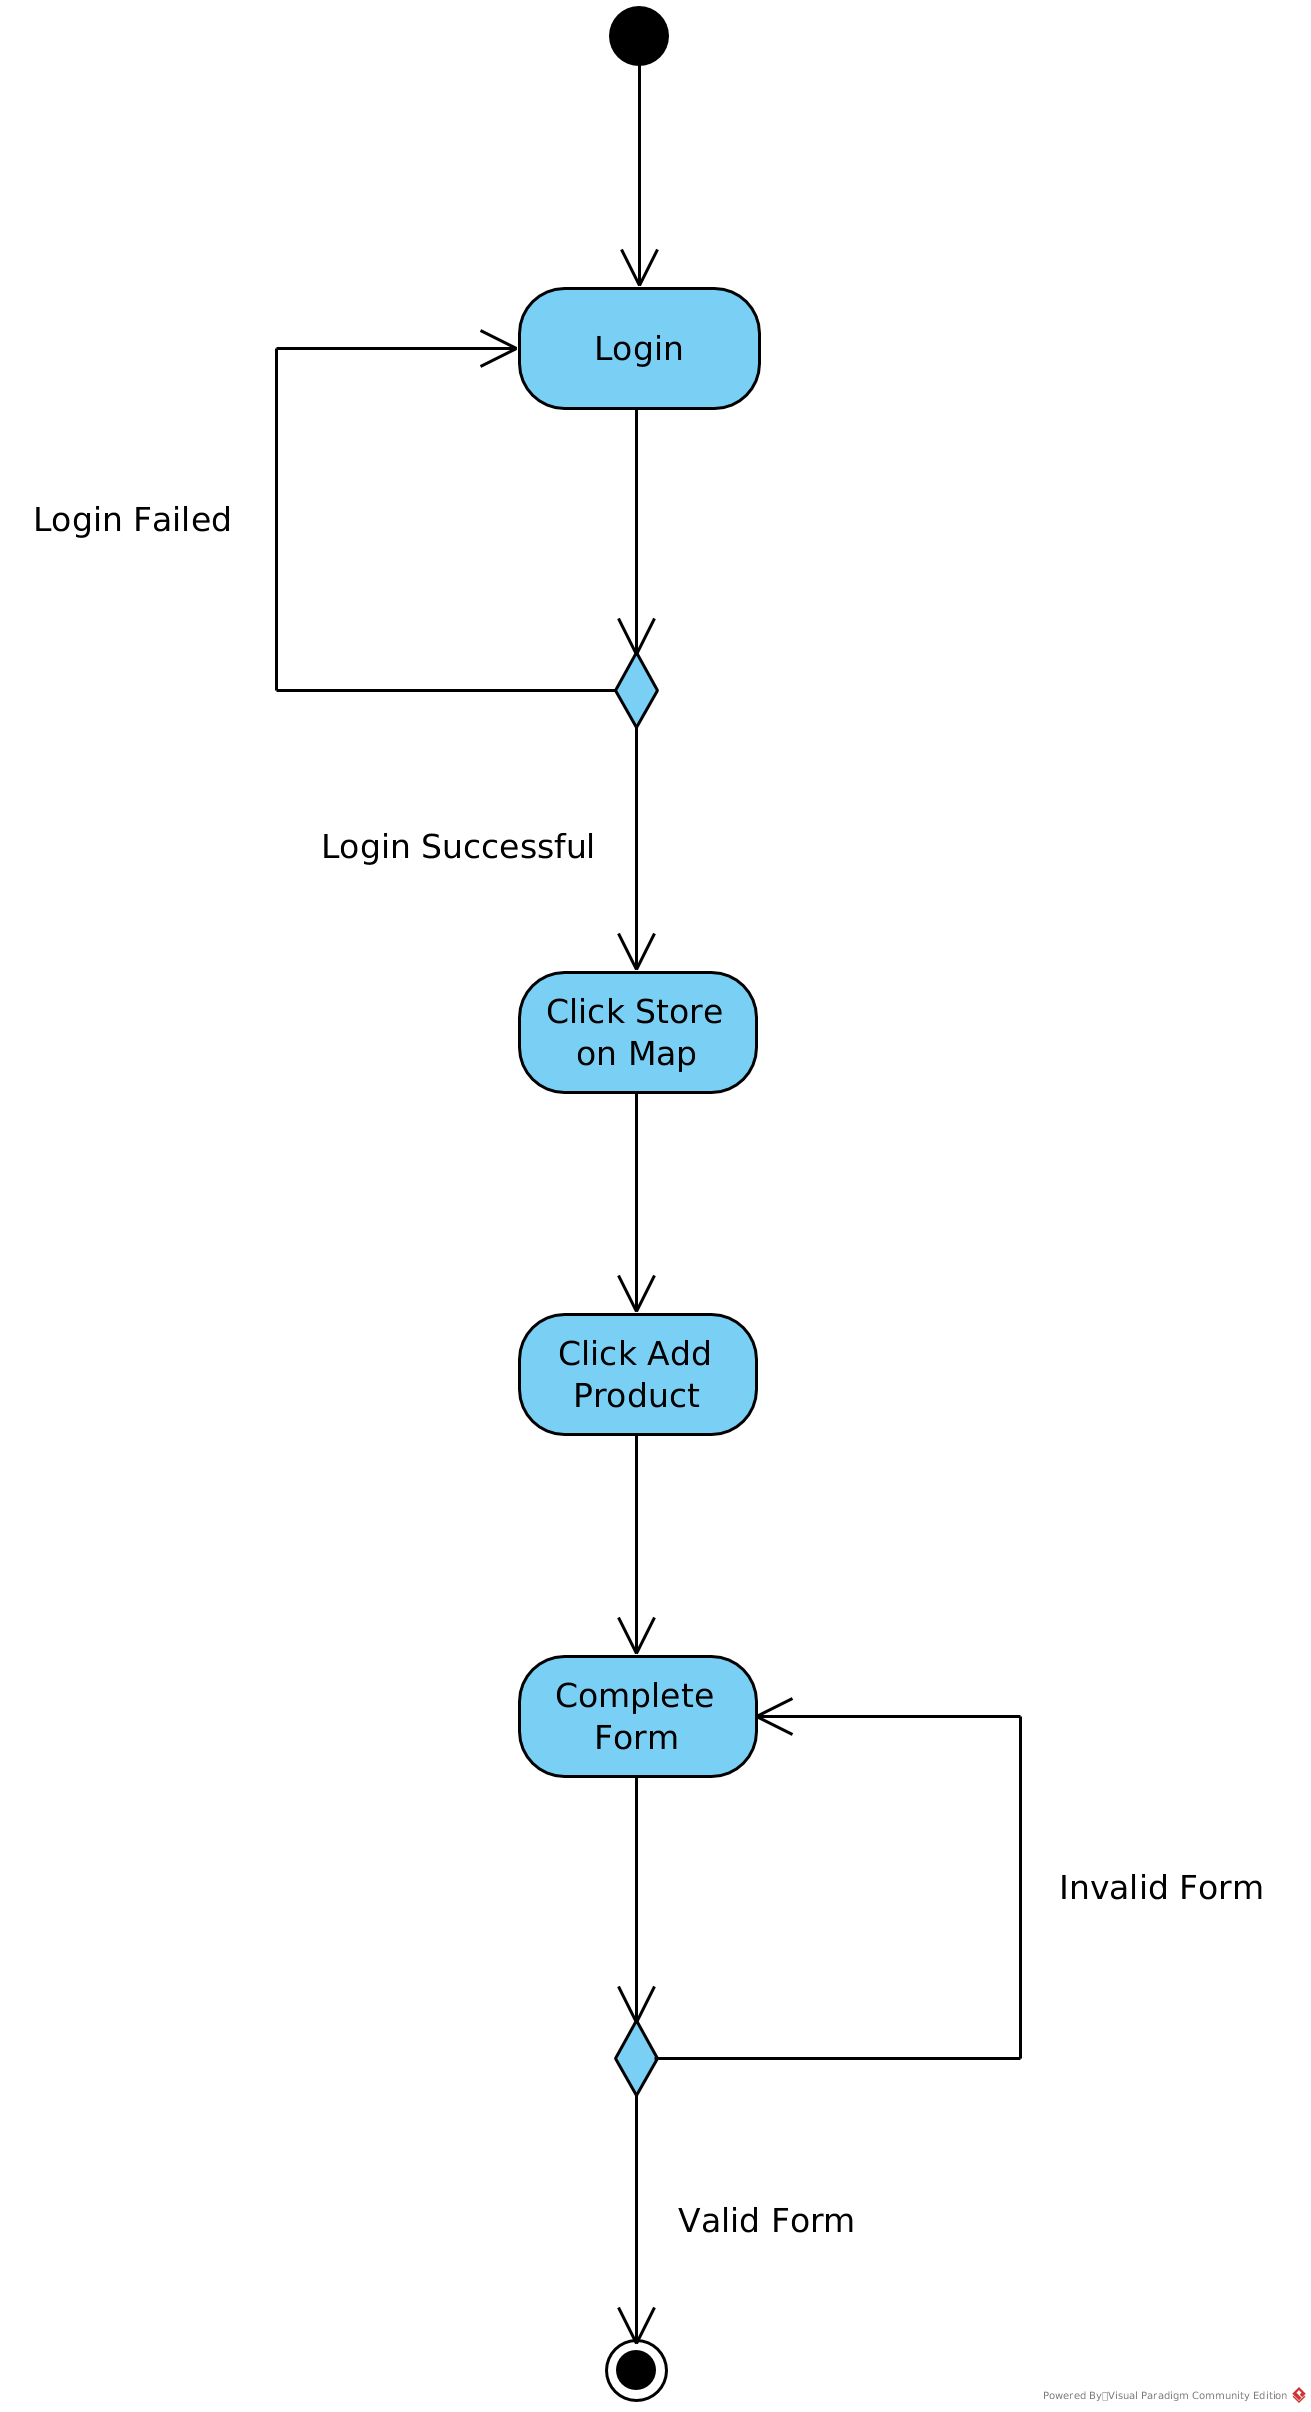
\includegraphics[]{media/Activity/User.png}
	\caption{User: Activity Diagram}
	\label{fig:User_Activity}
\end{figure}



\begin{figure}[H]
    \centering
    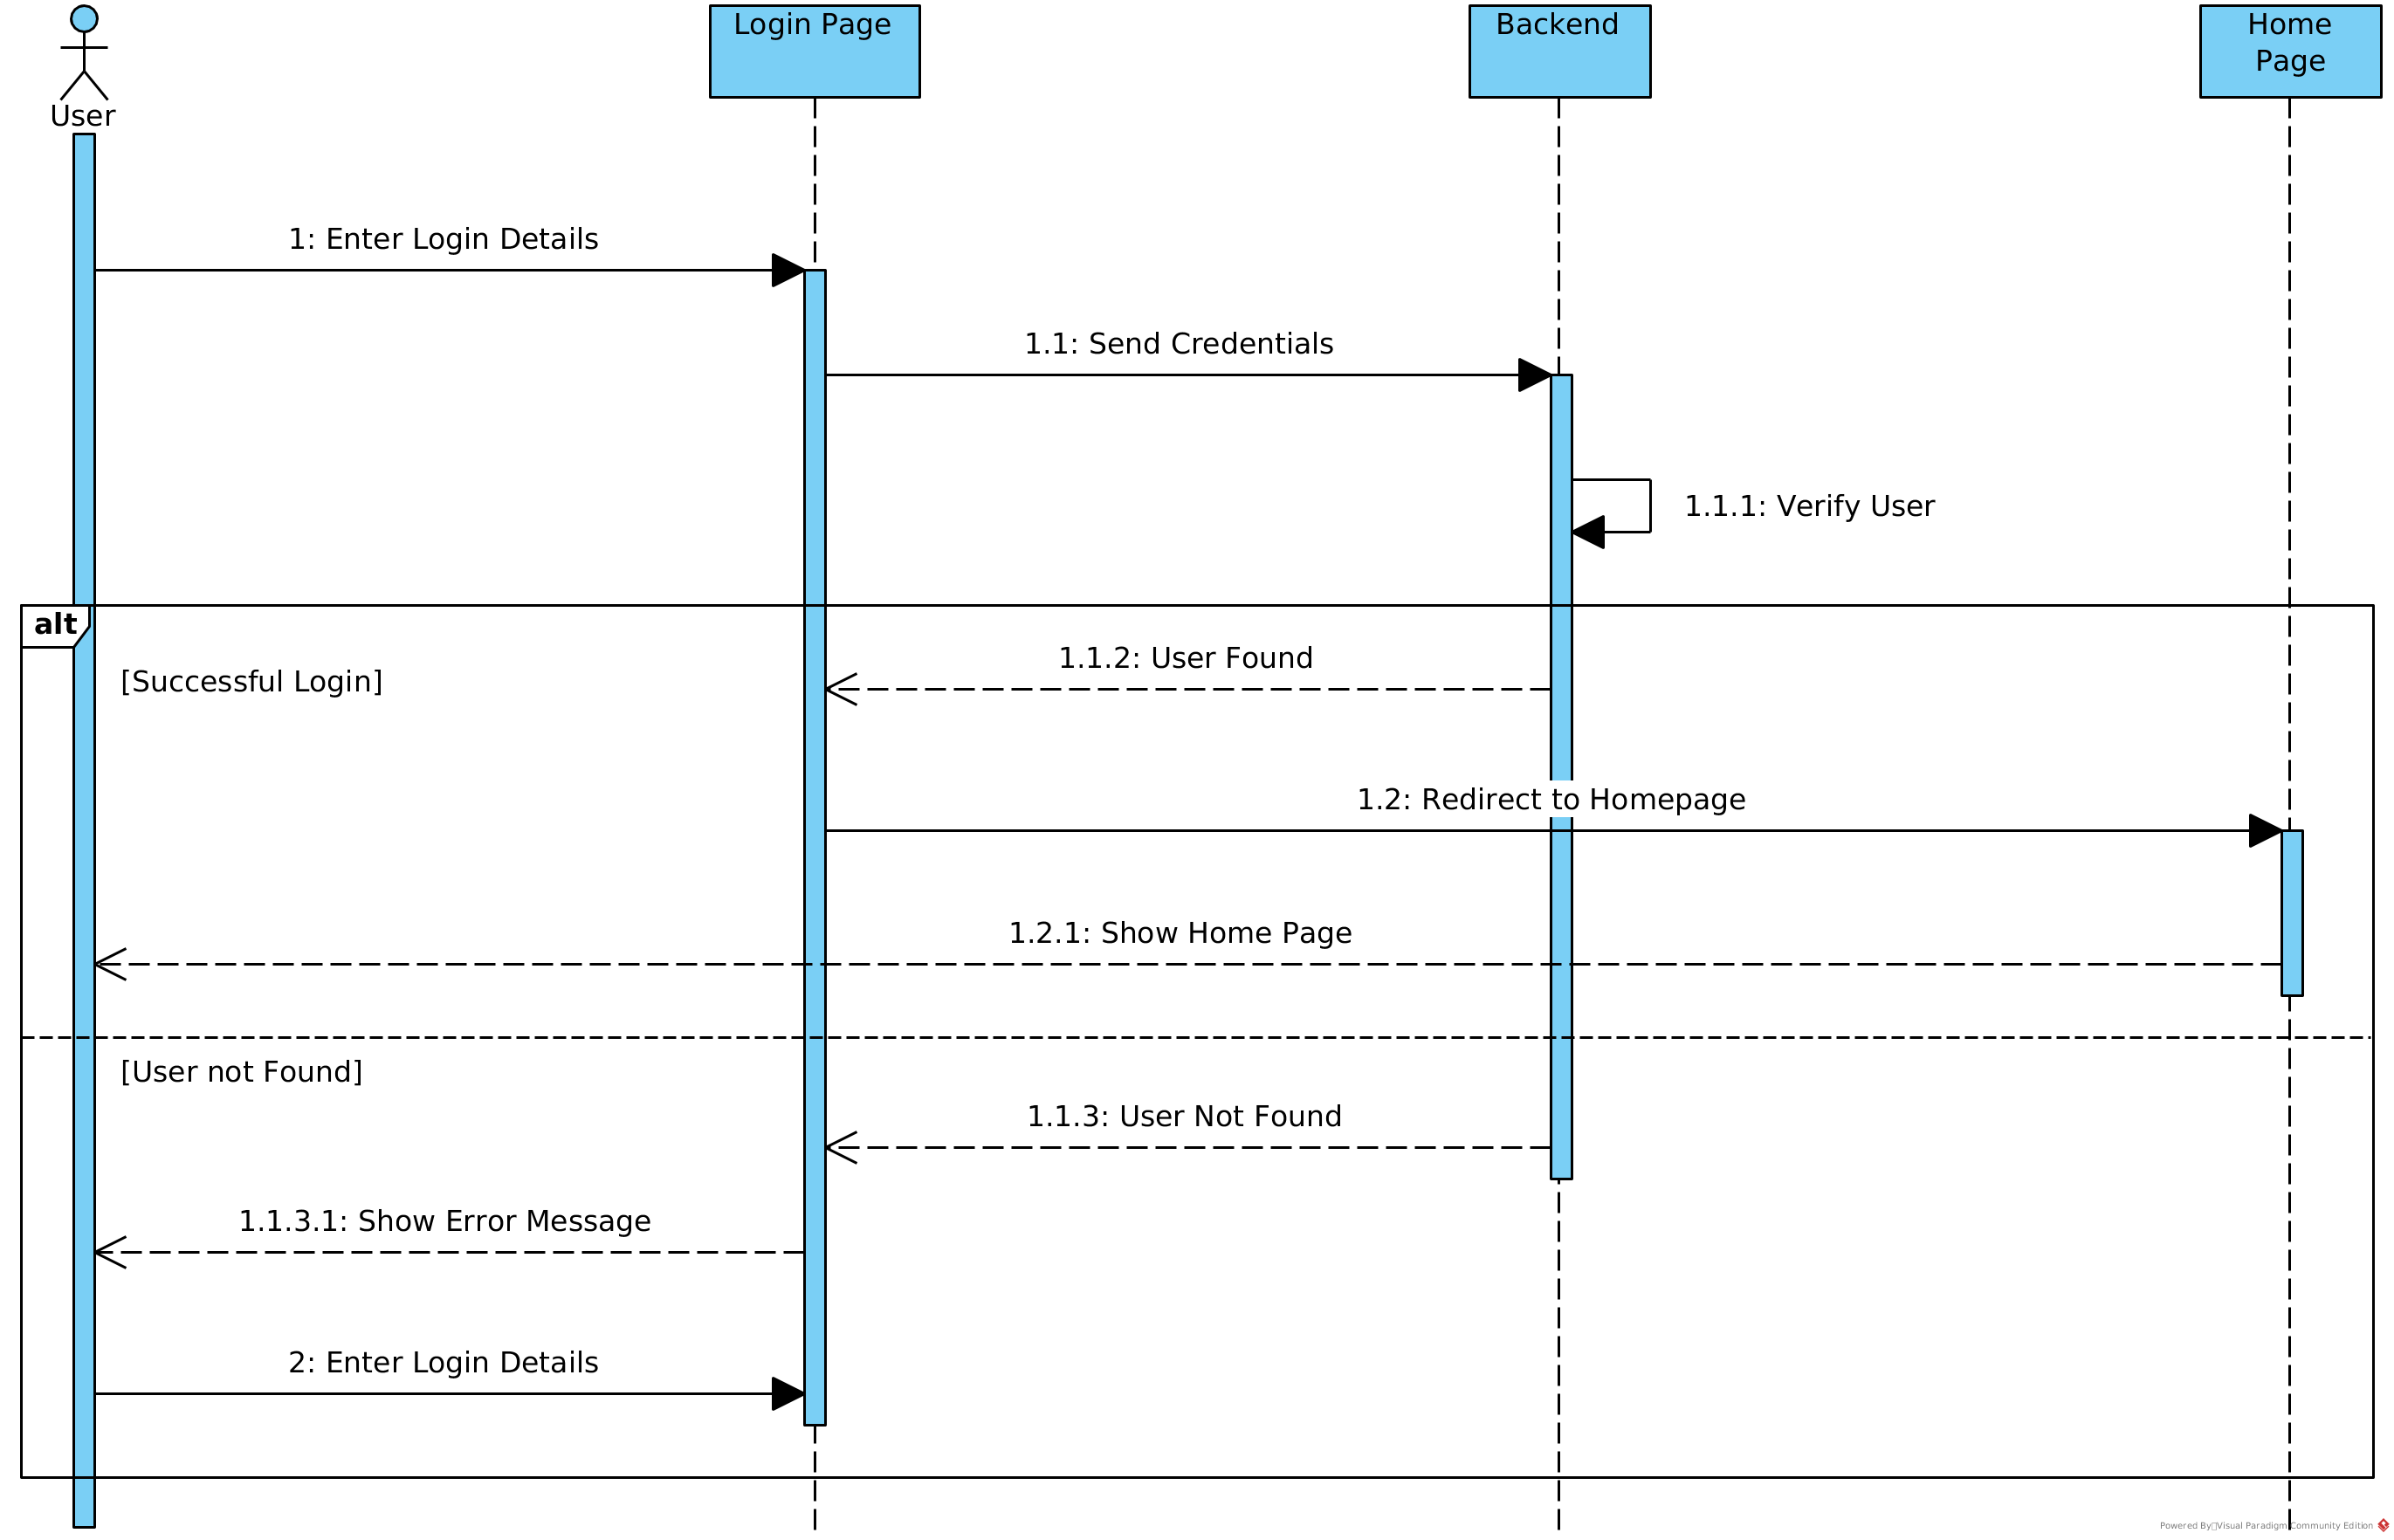
\includegraphics[width = \linewidth]{media/Sequence/User_Login.png}
	\caption{User Login: Sequence Diagram}
	\label{fig:User_Login}
\end{figure}


\begin{figure}[H]
    \centering
    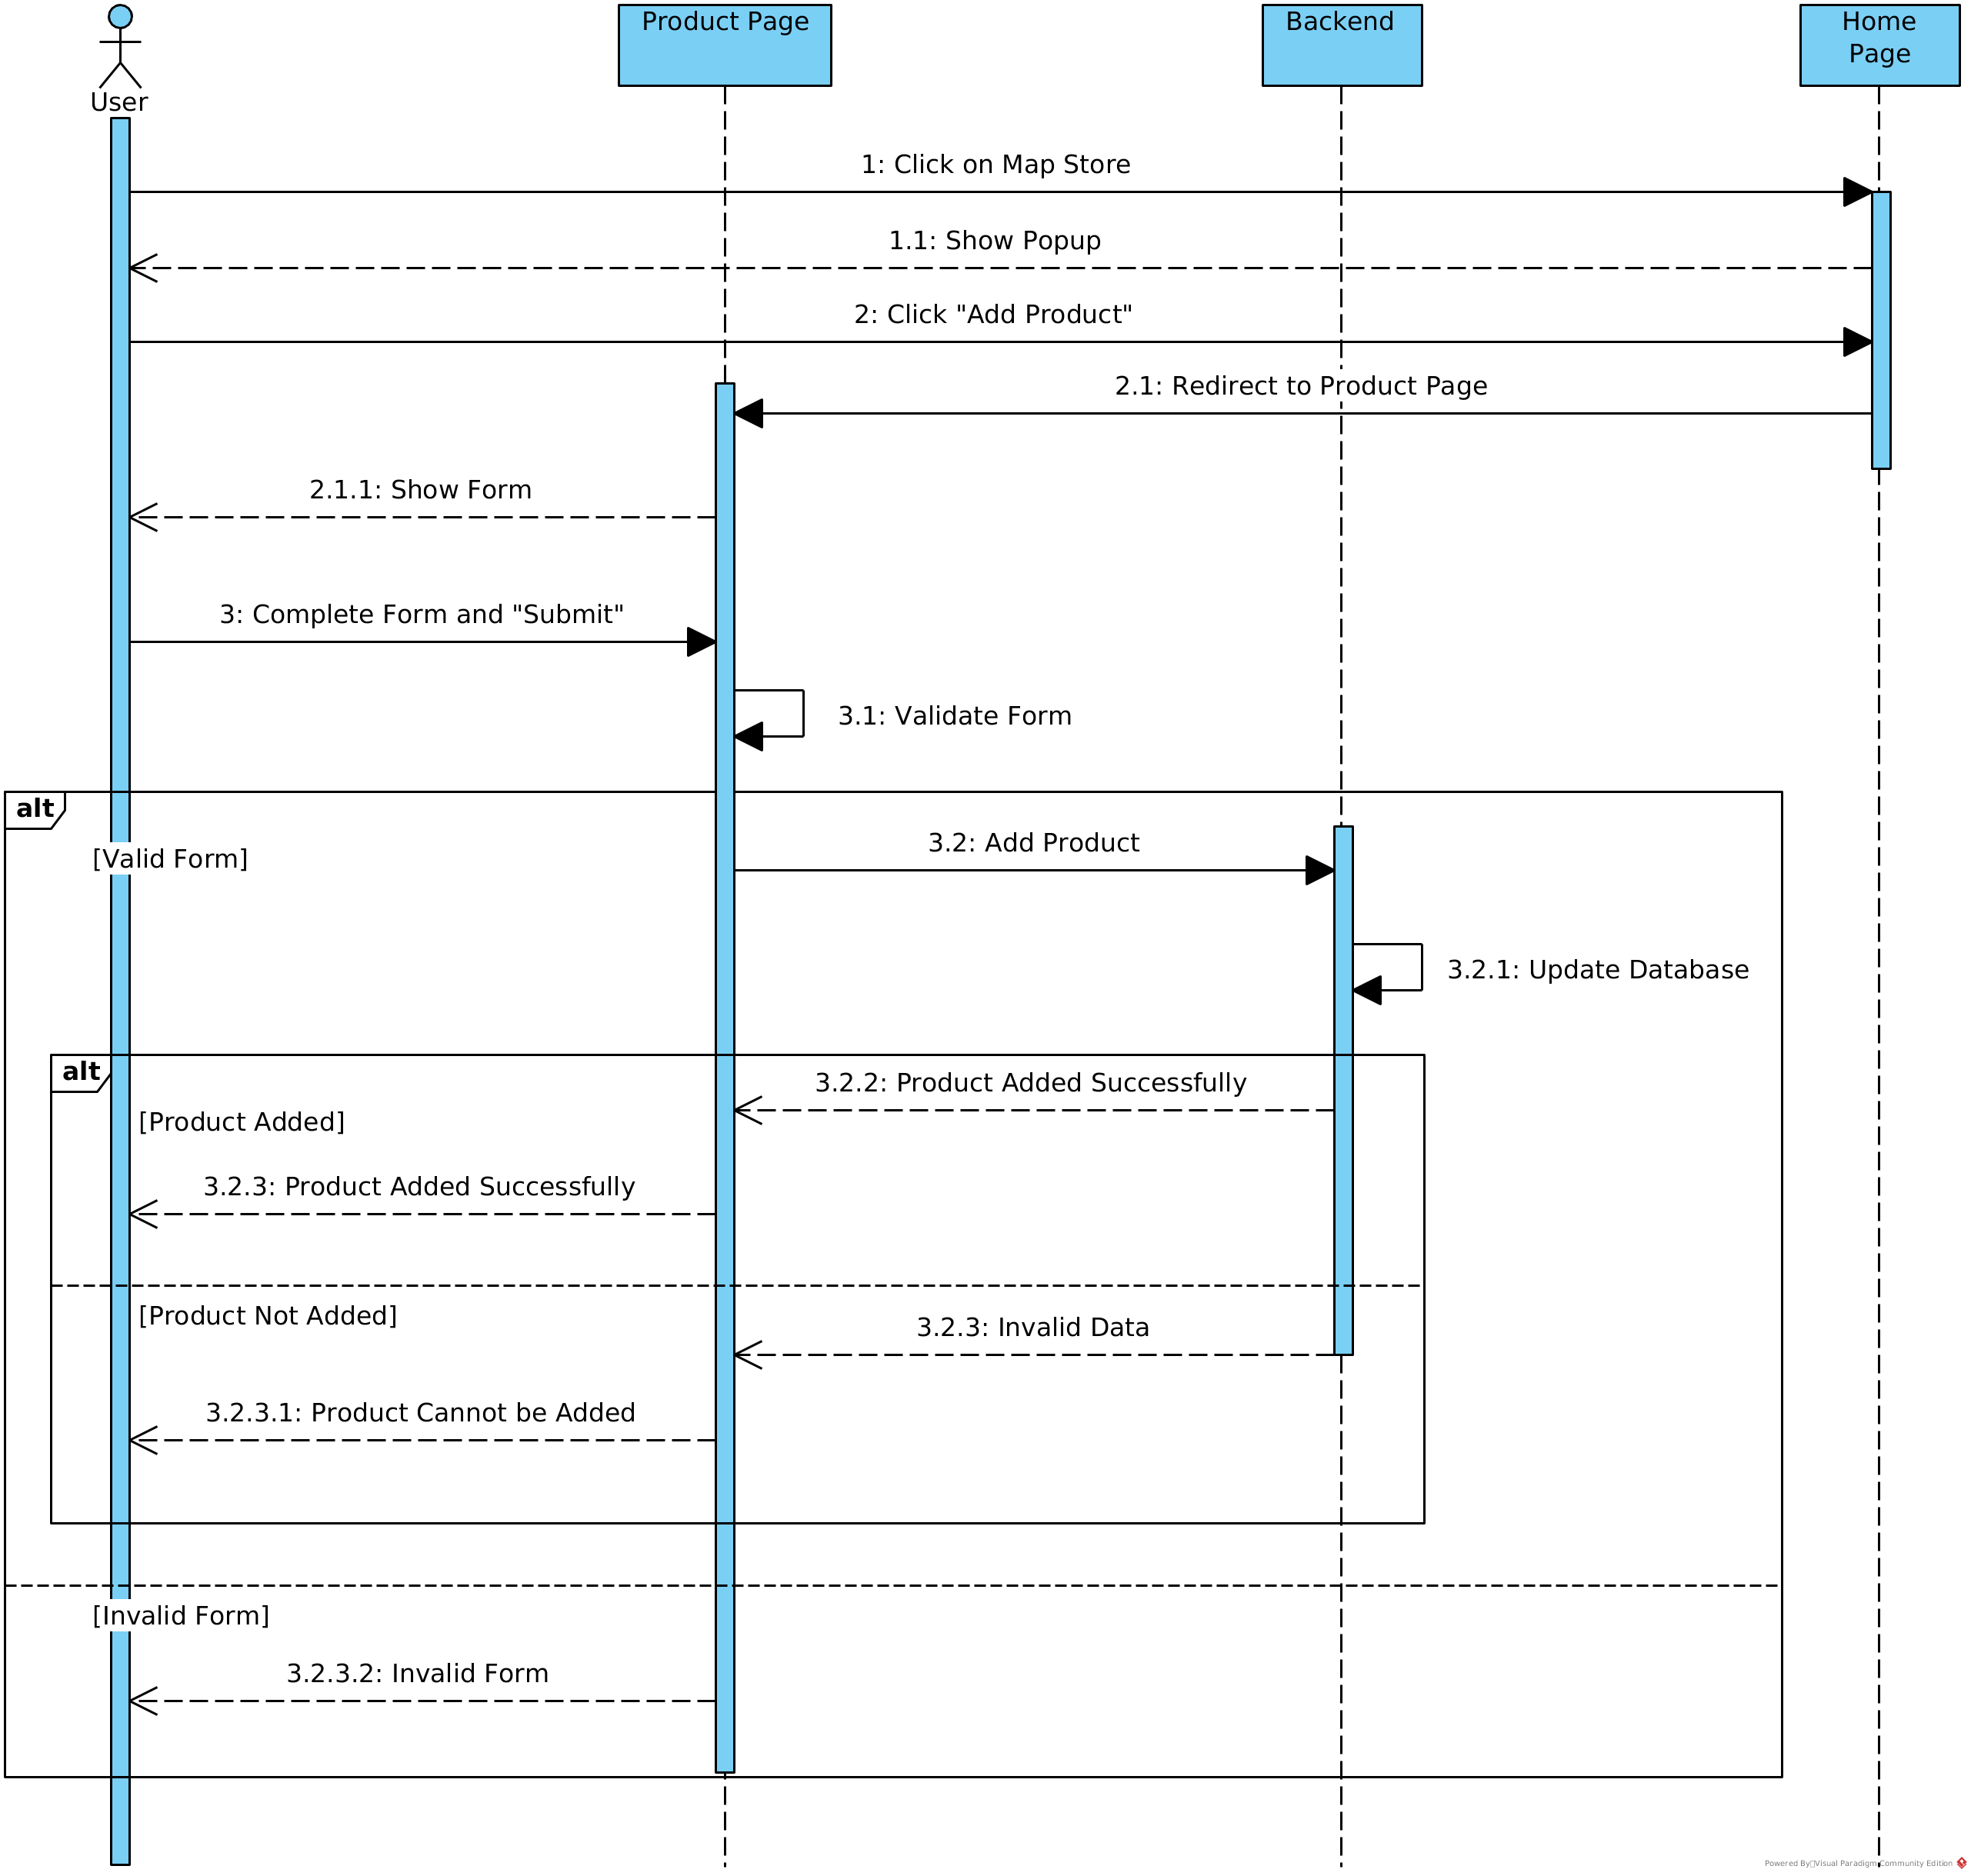
\includegraphics[width = \linewidth]{media/Sequence/User_Add_Product.png}
	\caption{User Add Product: Sequence Diagram}
	\label{fig:User_Add_Product}
\end{figure}

